The equation of circle can be expressed as
\begin{align}
    \vec{x}^T\vec{x}-2\vec{c}^T\vec{x}+f = 0
\end{align}
$\vec{c}$ is the centre  and substituting the points in the equation of circle we get
\begin{align}
2\myvec{-1&2}\vec{c}-f=5\\
 2\myvec{3&-2}\vec{c}-f=13\\
\myvec{1&-2}\vec{c}=0
\end{align}
can be expressed in matrix form
\begin{align}
\myvec{1&-2&0\\6&-4&-1\\-2&4&-1}\myvec{\vec{c}\\f} = \myvec{0\\13\\5}
\end{align}
Row reducing the augmented matrix
\begin{align}
\myvec{1&-2&0&0\\6&-4&-1&13\\-2&4&-1&5}
\xleftrightarrow[R_3\leftarrow R_3+2R_1]{R_2\leftarrow R_2-6R_1}
\myvec{1&-2&0&0\\0&8&-1&13\\0&0&-1&5}\\
\xleftrightarrow[R_1\leftarrow R_1+R_2]{R_2\leftarrow R_2/4}
\myvec{1&0&\frac{-1}{4}&\frac{13}{4}\\0&2&\frac{-1}{4}&\frac{13}{4}\\0&0&-1&5}\\
\xleftrightarrow[R_1\leftarrow R_1-R_3/4]{R_2\leftarrow R_2-R_3/4}
\myvec{1&0&0&2\\0&2&0&2\\0&0&-1&5}
\end{align}
\begin{align}
    \vec{c} = \myvec{2\\1}\\
    f = -5\\
    r=\sqrt{\norm{\vec{c}}^2-f} = \sqrt{10}
\end{align}
The required equation of circle is 
\begin{align}
\vec{x}^T\vec{x}-2\myvec{2&1}\vec{x}+5 = 0
\end{align}
See Fig. \ref{Fig:solutions4/1/5/}

\begin{figure}[!ht]
\centering
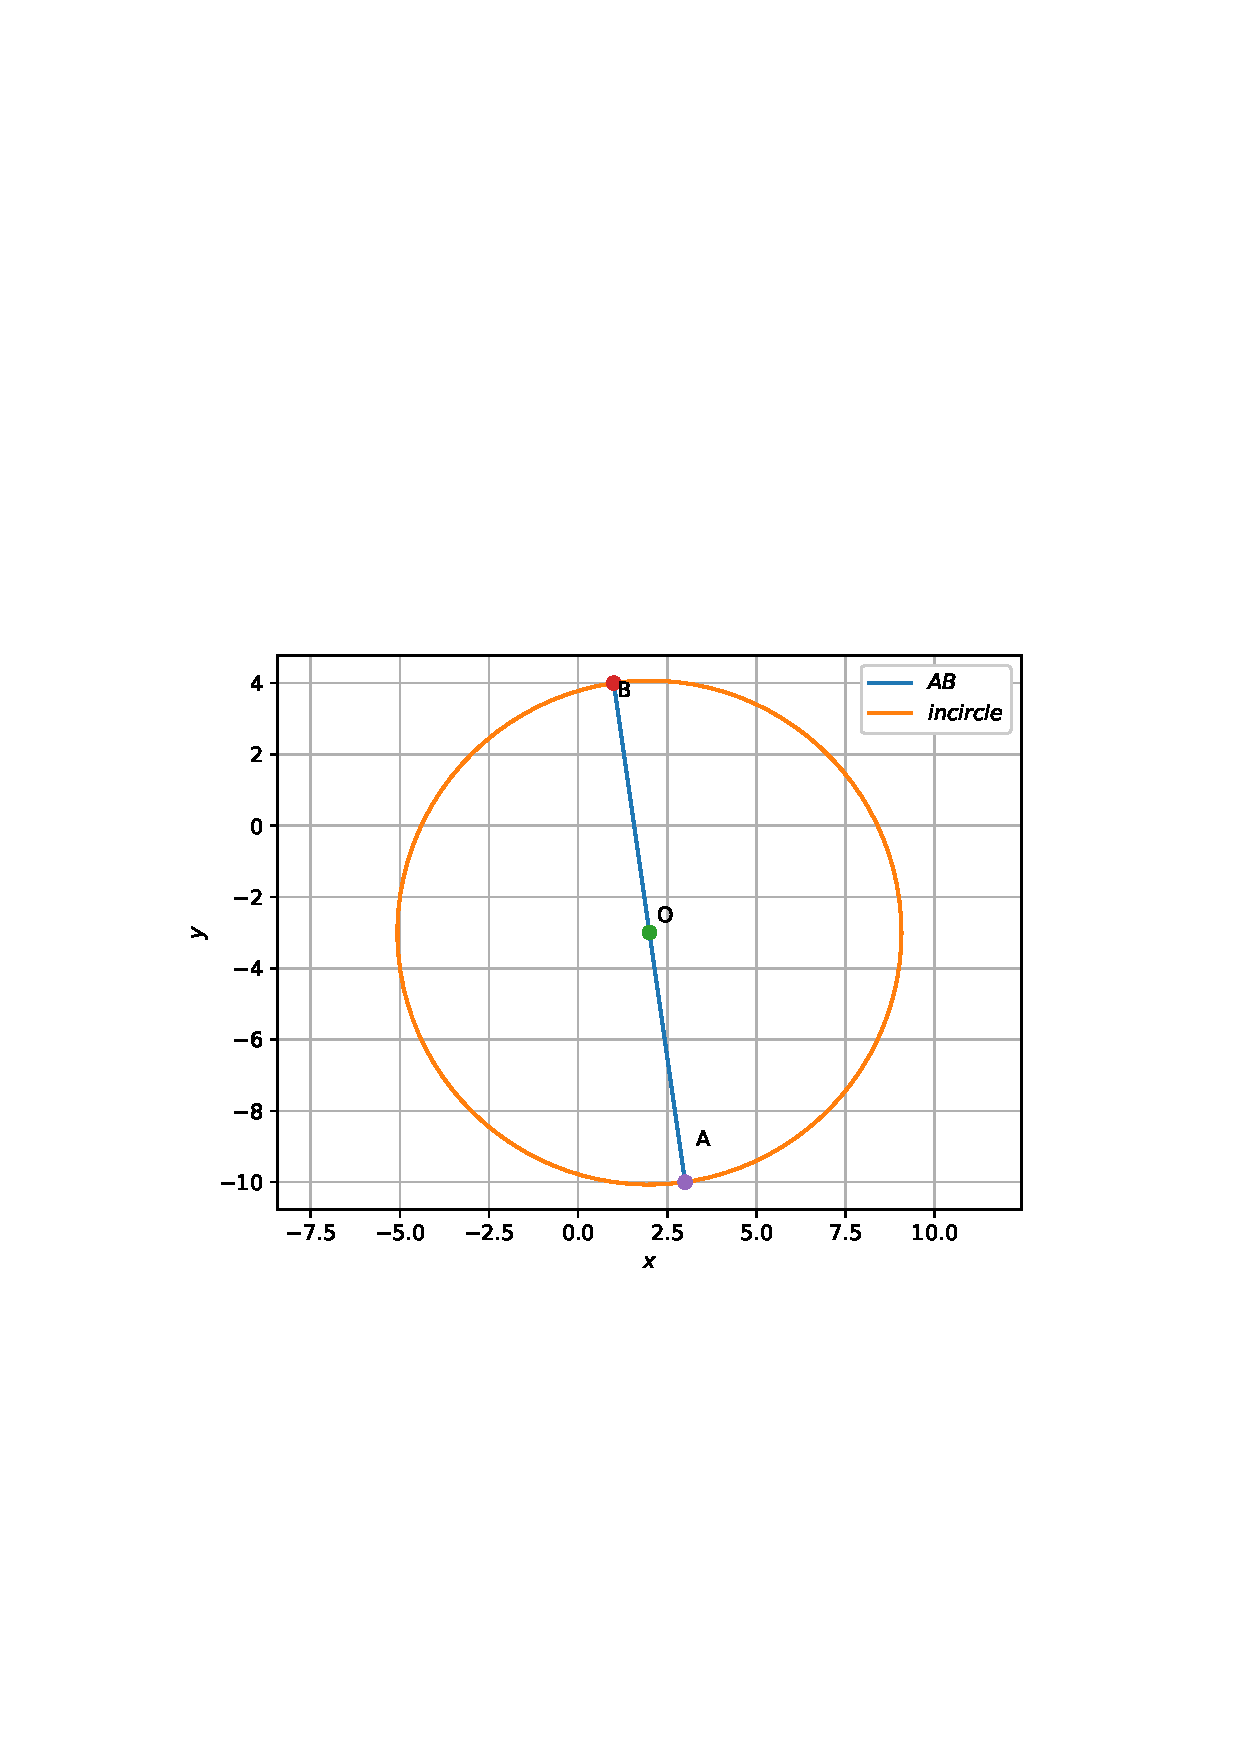
\includegraphics[width=\columnwidth]{./solutions/4/1/5/circle.png}
\caption{Circle passing through point P and Q also centre lie on the line x=2y}
\label{Fig:solutions4/1/5/}
\end{figure}
